\documentclass[12pt,a4paper]{report}

\usepackage[T2A]{fontenc}
\usepackage[utf8]{inputenc}
\usepackage[russian]{babel}

\usepackage{indentfirst}
\usepackage{graphicx}
\usepackage{amsmath, amsfonts, amssymb, amsthm, mathtools}

\author{
	Малов Андрей\\
	\and
	Школьник Савелий\\
}
\title{Описание программы}
\date{\today}

\begin{document}

\maketitle

\chapter{Проектная часть}
\section{Математическое обеспечение}

Вычисление степени нечеткого равенства осуществляется по следующим формулам:

\[f(x, a, b, c) = max(min(\frac{x - a}{b - a},\frac{c - x}{c - b}),0)\]

По формуле \(f(x,a,b,c)\) степень нечеткого равенства определяется методом принадлежности треугольника.  В данной формуле параметры \(a\) и \(c\) определяют начало и конец функции принадлежности, а \(b\) определяет её пик, а x --- значение принадлежности, заданное пользователем.

\[f(x, a, b, c, d) = max(min(\frac{x - a}{b - a},1,\frac{d - x}{d - c}),0)\]

По формуле \(f(x,a,b,c,d)\) степень нечеткого равенства определяется методом принадлежности трапеции. Параметры b и c определяют высоты функции принадлежности, а \(a\) и \(d\) определяют начало и конец функции принадлежности, а \(x\) --- значение принадлежности, заданное пользователем.
Форма функции принадлежности зависит от относительных значений \(b\) и \(c\):

\begin{itemize}
    \item Когда \(c\) больше, чем \(b\), функция принадлежности является трапециевидной.
    \item Когда \(b\) равно \(c\), функция принадлежности эквивалентна треугольной функции принадлежности c параметрами \([a, b, d]\).
    \item Когда \(c\) меньше \(b\), функция принадлежности является треугольной с максимальным значением меньше 1.
\end{itemize}

\section{Алгоритм работы программы}
\begin{enumerate}
    \item Привести все входные значения к нечетким функциям принадлежности и вычислить степень нечеткого равенства по формулам функций принадлежности. 
    \item Применить все правила в базе правил для вычисления нечетких выходных функций.
    \item Дефаззифицировать нечеткие выходные функции, чтобы получить «чёткие» выходные значения, то есть из полученного значения степени нечеткого равенства, которое будет принадлежать множеству [0;1] сделать вывод о степени близости параметра к оптимальному значению, например при оценивании погоды, используя степень нечеткого равенства мы можем получить значения 0, 0.5, 1 которые в четком виде будут соответствовать “плохая”, “умеренная”, “отличная” погода.
    \item После этих манипуляций над числами можно, основываясь на полученных значениях, будет осуществлен вывод в виде графика степени нечеткого равенства, состоящего из трех графиков, которые соответствуют отрицательному, умеренному и положительному прогнозам.
\end{enumerate}

\newpage

\section{Блок схема работы программы}
\begin{figure}[h!]
	\centering
	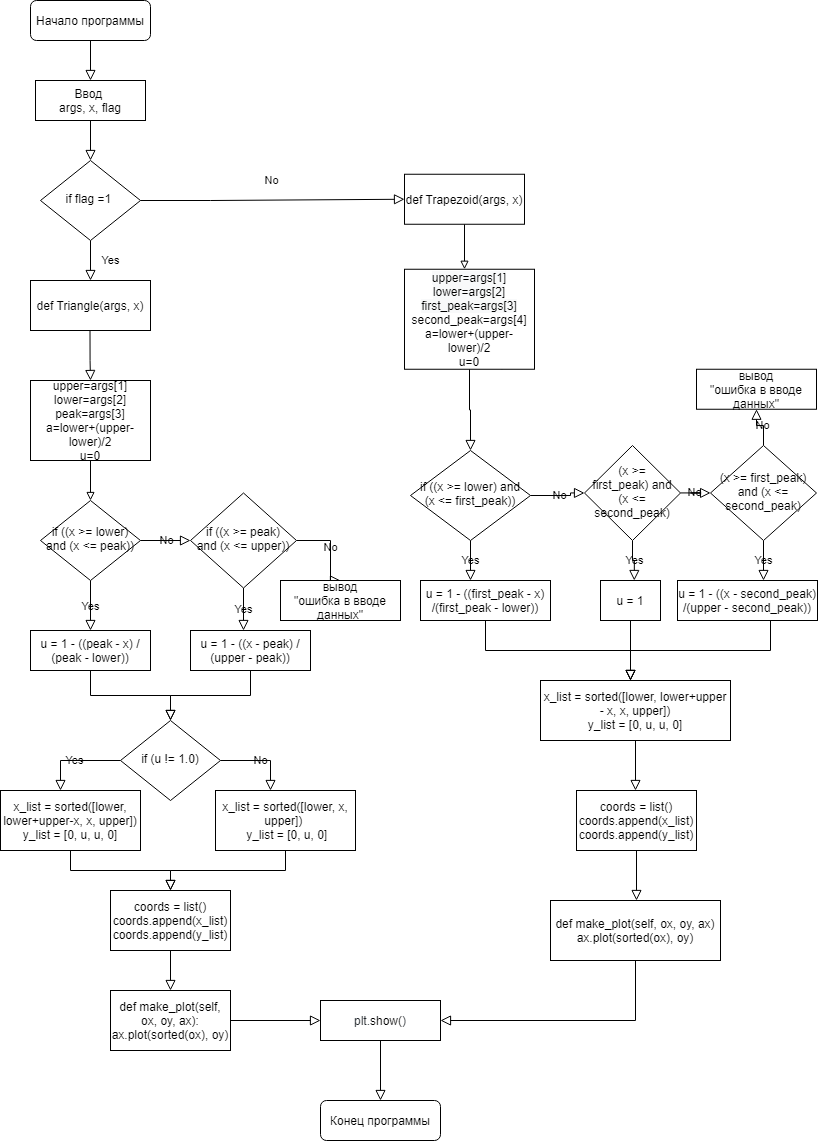
\includegraphics[width=0.95\textwidth, keepaspectratio]{diagram.png}
	\caption{Блок схема} 
\end{figure}

\section{Информационное обеспечение}
В данной программе входной информацией являются числовые данные как целые так и рациональные. Ввод не должен содержать дополнительных символов, таких как знаки препинания и буквы. Максимальная длина вводимого текста равна 100 символам. Текст вводится пользователем самостоятельно в консоли программы.

\section{Программное обеспечение}
В настоящее время существует огромное количество сред разработки
программного обеспечения. Каждая из сред программирования обладает
своими достоинствами. 

Python --- это интерпретируемый язык программирования общего назначения высокого уровня. Созданная Гвидо ван Россумом и впервые выпущенная в 1991 году, философия дизайна Python подчеркивает удобочитаемость кода с его заметным использованием значительных отступов. Его языковые конструкции и объектно-ориентированный подход направлены на то, чтобы помочь программистам писать понятный, логичный код для малых и крупных проектов.

Python динамически типизированный и имеет сборщик мусора. Он поддерживает несколько парадигм программирования, включая структурное (в частности, процедурное), объектно-ориентированное и функциональное программирование. Python часто описывается как язык «с батарейками» из-за его обширной стандартной библиотеки.

Python был задуман в конце 1980-х годов как преемник языка ABC. Python 2.0, выпущенном в 2000 году, появились такие функции, как списки и систему сбора мусора. Python 3.0, выпущенный в 2008 году, не полностью обратно совместим, и большая часть кода Python 2 не работает без изменений в Python 3.

Интерпретаторы Python доступны для многих операционных систем. Глобальное сообщество программистов разрабатывает и поддерживает CPython, эталонную реализацию с открытым исходным кодом.

\section{Библиотека в Python}
Большая стандартная библиотека Python, обычно упоминаемая как одна из ее сильных сторон, предоставляет инструменты, подходящие для многих задач. Для интернет-приложений поддерживаются многие стандартные форматы и протоколы, такие как MIME и HTTP. Он включает в себя модули для создания графических пользовательских интерфейсов, подключения к реляционным базам данных, генерации псевдослучайных чисел, арифметики с десятичными числами произвольной точности, управления регулярными выражениями и модульного тестирования.

Некоторые части стандартной библиотеки охватываются спецификациями, но большинство модулей - нет. Они определяются их кодом, внутренней документацией и тестовыми наборами. Однако, поскольку большая часть стандартной библиотеки является кроссплатформенным кодом Python, только несколько модулей нуждаются в изменении или переписывании для вариантов реализации.

По состоянию на ноябрь 2019 года Python Package Index (PyPI), официальный репозиторий для стороннего программного обеспечения Python, содержит более 200 000 пакетов с широким спектром функциональных возможностей, включая:
\begin{itemize}
    \item Автоматизация 
    \item Аналитика данных 
    \item Базы данных
    \item Документация 
    \item Графические пользовательские интерфейсы 
    \item Обработка изображений 
    \item Машинное обучение 
    \item Мобильное приложение 
    \item Мультимедиа 
    \item Сеть 
    \item Научные вычисления 
    \item Администрирование системы 
    \item Тестовые среды 
    \item Обработка текста 
    \item Веб-платформы 
    \item Веб-скрейпинг
\end{itemize}

\section{Построение графиков}
Для отрисовки графиков была использована библиотека для Python --- matplotlib.

Matplotlib --- это библиотека черчения для языка программирования Python и его числового математического расширения NumPy. Он предоставляет объектно-ориентированный API для встраивания графиков в приложения, используя универсальные наборы инструментов GUI, такие как Tkinter, wxPython, Qt или GTK +. Существует также процедурный интерфейс «pylab», основанный на конечном автомате (например, OpenGL), который очень похож на MATLAB, хотя его использование не рекомендуется. SciPy использует Matplotlib.

Pyplot --- это модуль Matplotlib, который обеспечивает интерфейс, похожий на MATLAB. Matplotlib разработан так, чтобы его можно было использовать так же, как MATLAB, с возможностью использовать Python и преимуществом свободного и открытого кода. К сожалению, на данный момент в среде С++ нет удобного и понятного аналога данной библиотеке, в связи с чем выбор рабочего программного обеспечения пал на язык Python - простой и понятный, многофункциональный и эффективный.


\end{document}
